\chapter{Testability of the solution}
This chapter describes the set of tests which are used to prove the quality of the code. The solution was designed for testability. In total there are five types of tests to stress the quality and correctness of the code.

\begin{itemize}
	\item  Standard unit tests to cover the business and data access layer.
	\item  Parametrized unit tests to increase the coverage of the business layer.
	\item  Unit test for ViewModels in the presentation layer.
	\item  Functional tests to test the whole application.
	\item  Load tests for performance analysis.
\end{itemize}

\section{Standard unit tests}
Standard unit tests were defined to verify the correctness of Data Access and Business layers. To isolate the tested code from the rest of the application Rhino Mock framework is used. See \ref{tech:unit} for the justification of this selection. In order to test the database persistence and the whole Data Access layer SQLite\footnote{\href{http://www.sqlite.org/about.html}{SQLite} is a embedded relational database framework, which runs without any separated server-side process. The data is stored in regular disk files.} database is used.

\section{Parametrized unit tests}
To exercise each path in the tested unit or method, several unit tests have to be written manually. For each of these tests the data has to be prepared and also the mocks prepared for each interacting component. This results in lot of repetitive code. This situation can be illustrated by the following code snippets. Assume that we have one method to test:

\begin{verbatim}
void Transfer(int creditId, int debitId, int amount) {}
\end{verbatim}

The above specified method uses the ID's of credit and debit accounts and adequate repository class to find these accounts. If both accounts were found, the method checks whether the transfer can be done. Some accounts may authorize the overdraft some not. This results in a set of tests:
\begin{itemize}
\item Credit and debit accounts are the same.
\item Credit account was not found.
\item Debit account was not found.
\item Amount is bigger than debit account balance and overdraft is not authorized. 
\item Amount is bigger than debit account balance and overdraft is authorized.
\item All parameters are correct
\end{itemize}
At least the 5 above mentioned tests should validate the method and make sure, that appropriate exception will be thrown when preconditions are not kept or other issues arise.

Parametrized unit tests are designed to simplify this situation. The signature of parametrized testing method will be usually the same as the signature of tested method. The parameters which are given to this method will vary. Parametrized testing framework can be used to automatically divine the parameters to exercise all paths in the method. In this solution Pex framework was used, which allows the creation of following parametrized unit test:

\begin{verbatim}
//a field which holds testing data
accounts = GetTestingAccountsData();

[PexMethod]
public void MakeTransfer(int debitId, int creditId, decimal amount)
{
    var repository = new SIRepository();
    
    //the repository will look up the accoun in testing data
    repository.GetObject<Account>((x) => 
    			accounts.SingleOrDefault(a => a.Id == (int)x));
	
    var operationServices = new OperationServices(repository);
    
    operationServices.Transfer(debitId, creditId, amount);
}
\end{verbatim}

Parametrized testing method initializes the target (\textit{OperationServices} class) and than passes the parameters to the tested method. A repository has to be given to the services class, in order to enable the service to find the accounts in the database according to the id's. In the code above the repository is mocked using \textit{SIRepository} mole class. This class is created using the Moles framework \ref{tech:moles}.

A delegates is passed to the \textit{GetObject} method which states that every time this method is called to look up an Account object in the repository, it will look the object up in a predefined field \textit{accounts} which can be any \textit{IEnumerable} object holding testing data.

Pex analyzes all the branches in tested method and initializes the parameters to cover each of the branches. Each of the set of parameters generated by Pex can than be stored as a new unit test. Instead of writing five unit testing methods, only one has to be written, assuming that Pex is able to generate the parameters. Section \ref{tech:parametrized_testing} discusses the technical details of parametrized unit testing using Pex framework.

\section{Unit testing the ViewModels}
One of the advantages of MVVM pattern is the ability to test the logic in the user interface. ViewModels are standard C\# classes however they reside in Silverlight assembly. Silverlight assemblies cannot be loaded into the Visual Studio test host environment. As the solution to this issue a specialized testing host environment is a part of Silverlight Toolkit. While using the Silverlight Toolkit, the tests can be written as standard unit tests. The only difference is that the tests are executed in the test host inside a web browser as a Silverlight XAP package.

The perimeter of the ViewModel testing is quite small, while all of the network calls have to be mocked and requires lot of boiler plate code. Most of the code of the ViewModels should also be tested by acceptance tests, therefor it is question to which extend the ViewModels should be tested two times (by unit as well as acceptance tests).

\section{Acceptance tests}
Acceptance test is a test which is conducted to determine if the requirements on the software are met\cite{wiki:acceptance}. In the context of software engineering project, it is useful when the tests are written by stakeholders with knowledge of the functional domain. The tests are usually written in business domain language. Acceptance tests are a sub-group of functional tests. Functional tests are black-box tests which are executed to determine the good functionality of the software. Acceptance tests are functional tests which also define concrete requirements based on the specification or contract.

Several acceptance testing frameworks exists which can be used to define the test in "easily understandable" language and executed automatically.

To define the tests on this solution FitNesse\footnote{FitNesse is a web server which translates functional tests from the form of wiki-pages to executable code.} was selected as an open source acceptance framework. However executing acceptance tests for Silverlight solution using FitNesse has several challenges.

The translation of human readable language to the acceptance tests is performed through Fixtures. Fixtures are simple classes having methods with "understandable" signatures, which are used to execute the application code. This is straightforward while developing server based web applications. In this situation the Fixtures invoke the server side code compiled in DLL (in case of .NET application) files or JAR files (in case of Java application). When the Model View Controller (MVC) pattern is used, than the Fixtures invoke the controller methods with parameters specified by the functional tests.

When using Rich Internet Application client such as Silverlight the situation is different. The code which should be invoked by the Fixtures are methods exposed by the ViewModels. Two facts complicate the situation. The ViewModel is separated from the server by network interface and all the service calls raising from the ViewModels are asynchronous. Figure \ref{fig:fitnesse_start} illustrates the situation.

The following snippet demonstrates a typical call to server side function represented in the ViewModel.

\begin{verbatim}

public ClientSideDTO MyObject {get;set;}
private IWCFService WCFService;

public GetObject(int id)
{
   WCFService.BeginGetObject(id,EndGetObject,null);
}

public void EndGetObject(IAsyncResult result)
{
   MyObject = WCFService.EndGetObject(resutl);
}
\end{verbatim}
The service which exposes "Begin-End" methods is usually generated by service generation tool based on the information exposed by the server. In the functional testing, this service should be replaced and call the methods directly inside server side DLL libraries.

\begin{figure}[h]
\begin{center}
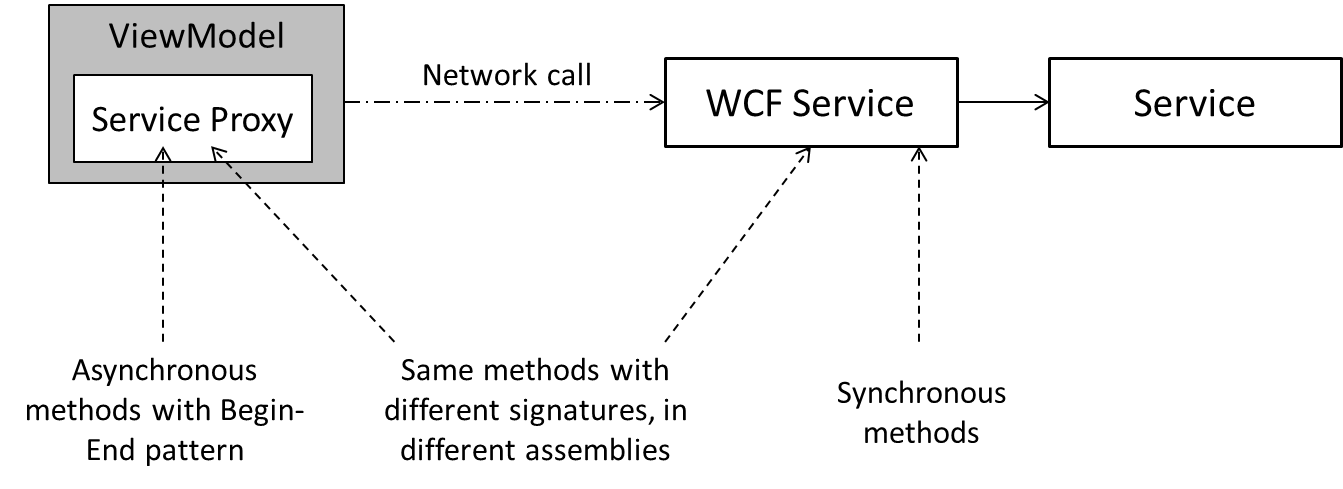
\includegraphics[width=14cm]{figures/fitnesse_start}
\caption{The issues of ViewModel calling exposed server side services}
\label{fig:fitnesse_start}
\end{center}
\end{figure}

There is a need for a architecture which would enable the use of server side services directly from the ViewModels. Also all the asynchronous calls will have to be "translated" to invoke the server side services directly.

The solution to this issue is the creation of wrapper class for the business layer, which can be injected directly to the ViewModel. The wrapper has to take care of the translation of begin - end combination to the call of business layer method and mapping between server side objects and client side objects. The architecture of the functional testing environment is demonstrated on figure \ref{fig:fitnesse_architecture}.

\begin{figure}[h]
\begin{center}
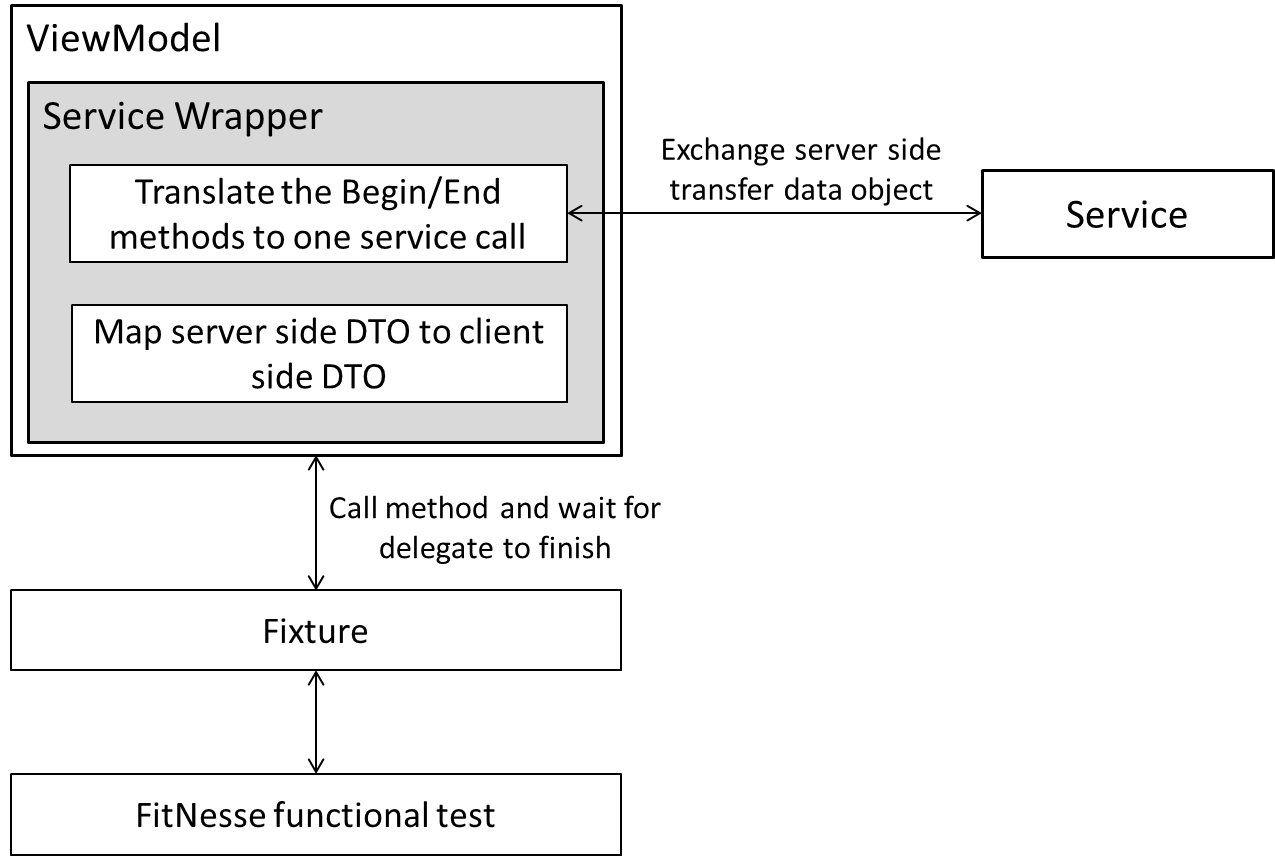
\includegraphics[width=14cm]{figures/fitnesse_architecture}
\caption{Infrastructure for functional testing}
\label{fig:fitnesse_architecture}
\end{center}
\end{figure}

The first step which has to be taken is the translation of "Begin - End" pattern to single method call. This can be achieved by introducing corresponding delegate, because any delegate offers the \textit{BeginInvoke} and \textit{EndInvoke} methods.

\begin{verbatim}
private IService service;

//delegate for a method which takes integer and returns ClientSideDTO
private Func<int, ClientSideDTO> Delegate;

ClientByID = (i) => {
    return Mapper.Map<ServerSideDTO, ClientSideDTO>(service.GetObject(i));
};
            
public IAsyncResult BeginGetObject(int id, AsyncCallback callback, object st)
{
    return Delegate.BeginInvoke(id, callback, st);
}

public ClientSideDTO EndGetObject(IAsyncResult result)
{
    return Delegate.EndInvoke(result);
}
\end{verbatim}

The business layer methods return server side DTO (Data Transfer Object) while the ViewModels work with generated client side DTO objects. These objects are the same, but do not reside in the same assembly, making the implicit conversion impossible. Explicit mapping has to be defined. This can be achieved thanks to auto-mapping libraries such as AutoMapper\footnote{\href{'http://automapper.codeplex.com/'}{AutoMapper} is an open source project generally dedicated to map values of one object to another, common situation which arises for example while converting data base entity object to data transfer object.}. In the above presented snippet, the delegate which calls server side services also uses the \textit{Mapper} class of AutoMapper to make the conversion of server side to client side object.

The last issue comes from the asynchronous nature of the methods in ViewModel. FitNesse has to make assertions after the execution of the operations. However if an assertion follows directly after the \textit{BeginOperation} method, it will be executed before the callback was finished and probably fail.

One option would be to introduce synchronization logic into the callback method. However the callback method is standard part of ViewModel and it would not be wise to increase the complexity of ViewModel for the reason of FitNesse testing.

The possible solution is a combination of signaling and active waiting. The \textit{BeginOperation} method returns \textit{IAsyncResult}. This standard .NET interface contains waiting handle, which signals the end of asynchronous operation. Unfortunately the same signal is send to the callback and starts the execution of the callback.

However all the operations of ViewModel use boolean variable \textit{InProgress} which signals the execution and ending of asynchronous methods. This variable is set to \textit{false} at the end of each \textit{EndOperation} method and thus can be used for active waiting.

Since the active waiting is executed after the signal has come about the termination of asynchronous operation, it is surely after the variable has been set to \textit{true} in the \textit{BeginOperation} method. The use of signal evicts the race conditions which could arise while using only active waiting for \textit{InProgress} variable.

\begin{verbatim}
var customerVM = new CustomerViewModel();

//wrapper instead of real service proxy
customerVM.CustomerService = new CustomerServiceWrapper(_customerServices);
var result = customerVM.GetObject(customer.Id);

//wait for the asynchronous operation to finish
result.AsyncWaitHandle.WaitOne();
result.AsyncWaitHandle.Close();
while (customerVM.InProgress == true) Thread.Sleep(20);

//the customerVM is ready and all service calls have finished
\end{verbatim}

The functional tests (or acceptance tests) prove the correctness of all layers of code. This is a possible advantage over unit tests, while unit tests are isolated to test only one feature. Also the amount of code which has to be written for isolation of unit tests exceeds the amount of code needed for preparation of fixtures. Once the fixtures are prepared business analysts can write the acceptance tests.

\section{Load tests}
Simple usage scenario was defined to obtain metrics about the application deployed to Azure platform.

\begin{itemize}
	\item Client logs into the applications
	\item Client checks the accounts and operations performed on the accounts during last six months. In total the client has 2 accounts, each having 120 categorized transactions.
	\item Client loads to view 5 business partners and personal tags.
	\item 20 client profiles are loaded with tag's repartition, which client can use to make comparison.
\end{itemize}

The test was defined using Fiddler web debugger and StresStimulus plug-in \footnote{Fiddler is web debugger which monitors the HTTP network traffic. Fiddler alone or with plug-ins can be used to analyze the HTTP requests. StressStimulus is a load testing tool available as plug-in for Fiddler. It enables recording and re-execution of HTTP requests. It provides also the possibility to parametrize the requests and define different load strategies}.

The scenario was executed for one client. Figure \ref{tab:metrics_one} provides the obtained metrics. To perform the simulation the network was limited to Dial-Up 56k modem to limit the quality of local connection on the test. Thus the download speed was 56.0 kbit/s and upload speed 33.6 kbit/s.

\begin{table}
\begin{center}
\begin{tabular}{|c|l|}
\hline
Total send bytes & 29792 \\
Total received bytes & 90135 \\
Total HTTP requests & 32 \\
Response time one one request & 1.59 s \\
\hline
\end{tabular}
\end{center}
\caption{Metrics of one execution of typical usage scenario}
\label{tab:metrics_one}
\end{table}

The same scenario was executed again in 60 iterations. During each iteration 5 new clients would ask the same resources. At each second new iteration was executed. After all 60 iterations, the test waited for the requests to finish. Figure \ref{tab:metrics_300} gives the metrics obtained by the execution.

\begin{table}
\begin{center}
\begin{tabular}{|c|l|}
\hline
Number of iterations & 60 \\
Number of users per iteration & 5 \\
Total bytes sent & 1795556 \\
Total bytes received & 5394520 \\
Average response time & 1.85 s \\
Bytes sent per second & 13349 \\
Bytes received per second & 40106 \\
Total number of HTTP requests & 1920 \\
\hline
\end{tabular}
\end{center}
\caption{Metrics obtained by repeated execution of typical use case scenario}
\label{tab:metrics_300}
\end{table}